\documentclass[a4j]{jarticle}
\usepackage[dvipdfmx]{graphicx}
\usepackage{eclclass}
\usepackage{url}


\setlength{\headsep}{-5mm}
\setlength{\oddsidemargin}{0mm}
\setlength{\textwidth}{165mm}
\setlength{\textheight}{230mm}
\setlength{\footskip}{20mm}

\title{
\vspace{30mm}
{\small 学生支援システム} 
\\
\vspace{5mm}
{\bf システム提案書\\}
\vspace{5mm}
{\small 第1.0版}
\vspace{90mm}
}

\date{\today}

\author{
\vspace{5mm}
  若草色.inc
\vspace{10mm}
}

%date{
%平成28年4月17日
%}

\begin{document}
\maketitle

\newpage


\section{はじめに}

学生が快適な学生生活を送るためには、手軽に自身の履修状況を把握することが求められます。
また、学校からの連絡などを正確かつスムーズに受け取る環境も求められます。
しかし現状では、履修状況や連絡事項の確認を手軽に行うことが実現しておらず、
授業教室の変更や提出期限の連絡などを把握していない学生がいます。
今回は、これらの問題を解決するための方法を提案をさせていただきます。

私達が提案する内容は、学生の履修状況や学校からの連絡を行うシステムと連携するアプリケーションを学生に提供することです。
これにより、学生がスマートフォンを用いて、履修状況や学校からの連絡などを容易に確認できる環境を実現します。また、スケジュール管理を容易に行えるため、学生生活のサポートに繋がると考えております。


\section{解決できる経営課題}
%アンケートを行った結果、現在のシステムに不満を持っている人がいることが分かりました。既存のシステムではオンライン状況でしか既存のシステムにある情報を確認できません。その為、オフライン上で更新された履修状況を確認できる様に、アプリ内での情報保持を行う事でネットワーク経由でのアクセスを行う必要が無いと言ったメリットがあります。\\
%また、履修状況のスケジュール管理を行える様になる事で、授業への遅刻・欠席が減り、学生の授業参加率を向上させる事が可能になります。
%(別府)具体的な数値がなく、グラフを貼るわけでもないのにアンケートのことをのべるのはどうかと、あと解決策をのべるところなのか微妙。
学生は、自身の履修状況や学校からのお知らせを確認し、それに合わせた生活を送らなければなりません。しかし、高知工科大学生を対象に実施したアンケート結果では、既存のシステムに対して不満を持っている人が半数以上確認され、より便利な機能を欲する声も多く挙げられました。\\
 また、Web上のシステムを利用するには、オンライン状況でアクセスを行うという前提が存在します。そのため、回線速度が遅い、ネットワークが混み合っているなどといった不安定な通信状況下では、自身のスケジュールやお知らせを確認することが困難です。この課題の要因には、「月ごとのデータ使用量の超過」や「同時刻におけるシステムへのアクセス数の多さ」などが挙げられます。\\
 前者は学生が自身の携帯端末を使用した時に限られますが、通常、多様な情報を取得するために使用している人々も多く存在するため、システムの円滑な利用にあたって、携帯端末からのアクセスを考慮に入れる必要があります。後者に関しては、ある程度の時間経過を待つことによって解消される可能性もありますが、緊急の場合に対応できないという問題点があります。\\
 したがって、従来、学生に提供されているシステムだけでは、学生が自身のスケジュール管理を行い、より快適な学生生活を送るための支援として不十分であると考えられます。


\section{課題解決のための提案}
本提案書では既存学生支援システムの学生向け情報閲覧のためのAndroidアプリシステムについてご提案いたします。


既存の学生支援システムと連携したAndroidアプリを作成し、このシステムを利用している学生がこのアプリをスマートフォンにダウンロードすることで、容易に情報の閲覧を行うことができます。


\section{課題解決のための方法}
前項で説明した事柄に関して、具体的な方法を以下に示します。
%\begin{itemize}
%\item 既存学生支援システムに対応したAndroidアプリケーション
%\item Androidアプリケーションとサーバの連携システム
%\end{itemize}
\begin{itemize}
\item 簡易な情報取得\\
 個人情報の保護のための認証機能は、指紋認証など端末に付随されている認証技術を利用します。アプリにおいて、一度ログインされたアプリはログアウトされるまで、その人物に関する情報を保持します。これにより、セキュリティ上、毎回行われるIDやパスワード認証を実施せず、素早い情報取得を実現します。
  %携帯の指紋認証とかされてるから、ある程度のセキュリティは確保されているよねってくだりをどこかに入れたかった。
\item 他Webサイトへの遷移\\
 これは、授業内容や書類提出先など学生に関連した他Webサイトに対して、Webブラウザ上の該当ページを表示するリンクなどを付属し、それらの情報取得を容易にするための項目を提供します。
\item ネットワーク環境に依存しない同情報取得\\
 このアプリは、以前にアクセスした際のデータを端末側に保持し、不安定なネットワーク状況下においても、前回アクセスした内容と同等な情報取得を可能にします。
\end{itemize}


\section{機能概要,前提条件}
\subsection{機能概要}
このAndoroidアプリでは以下の機能を導入します。\\ \\
(1)当日の授業情報\\
\hspace{5mm}
\begin{minipage}[h]{145mm}
 当日から翌々日までの時間割をトップページから、確認できます。
\end{minipage}
\\ \\
(2)履修登録情報\\
\hspace{5mm}
\begin{minipage}[h]{145mm}
 Web上で登録しておいた履修情報の一覧が確認できます。
\end{minipage}
\\ \\
(3)成績\\
\hspace{5mm}
\begin{minipage}[h]{145mm}
 自分の成績を確認できます。成績の表示は「科目区分別単位修得状況」「年度・学期別単位修得状況」「期間GPA」の3つの表示方法を選択できます。
\end{minipage}
\\ \\
(4)お知らせ\\
\hspace{5mm}
\begin{minipage}[h]{145mm}
 学校からのお知らせを閲覧できます。お知らせごとに項目分けしています。
\end{minipage}
\\ \\
(5)リンク\\
\hspace{5mm}
\begin{minipage}[h]{145mm}
 学校の関連ホームページをブラウザで開くことができます。リンクは「シラバス」「KUTLMS」「WebMailService」の3つです。
\end{minipage}
\\ \\
(6)テストカウントダウン\\
\hspace{5mm}
\begin{minipage}[h]{145mm}
 手動で設定しておくと、テストまであと何日かを表示してくれます。
\end{minipage}
\\ \\
(7)設定\\
\hspace{5mm}
\begin{minipage}[h]{145mm}
  このアプリのテストカウントダウン機能の設定と画面の見た目の設定ができます。
\end{minipage}

\subsection{前提条件}
このシステムは以下を前提条件とします。
\begin{itemize}
\item 4クオータ制を導入している学校を対象とする
\item 作成したアプリを既存システムを利用している学生にインストールしてもらう
\end{itemize}


\section{情報の流れ}
\begin{figure}[h]
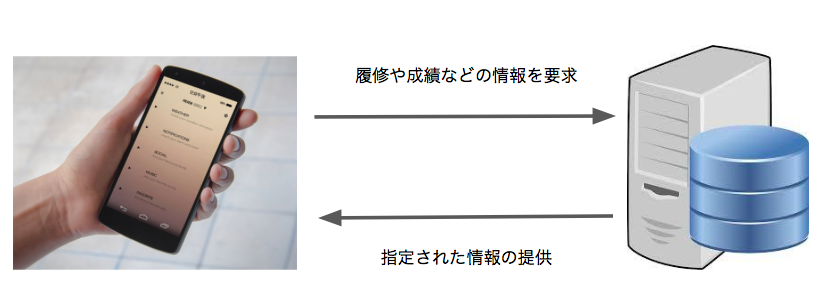
\includegraphics[scale = 0.5]{./nagare.png}
\caption{情報の流れ}
\label{flow}
\end{figure}

システムとしては,まず大学PCで使用されているユーザ名とパスワードを用いて登録してもらいます。その後、その日の講義一覧やお知らせ、成績などが閲覧できるアプリとなっています。Web上で履修を変更した場合にも、即時反映できるようになっています。


\section{想定する利用者}
このシステムの想定する利用者は次の通りです。
\begin{itemize}
\item 学生:Android端末を所持している生徒
  \end{itemize}


\section{システムのハードウェア,ソフトウェア構成}
中心サーバ:1台


\section{導入・移行計画}
2017年1月15日を持って、このシステムを導入します。


\section{運用・保守}
\begin{minipage}[h]{150mm}
(1)通常時の運用は、管理者が行います。\\
(2)故障発生時には、保守会社が行います。\\
(3)システムの運用スケジュールは以下の通りです。\\
\end{minipage}

\hspace{1cm}
\begin{minipage}[h]{140mm}
日〜火曜,木〜土曜 終日,水曜 午後\\
\hspace{5mm}
ログイン機能、データベースのシステム稼働\\
水曜 午前\\
\hspace{5mm}
メンテナンス(システム停止) \\
\end{minipage}


\section{作業標準}
システム開発に掛かる作業標準は御社ご指定のものを使用します。


\section{品質管理}
システム開発に掛かる品質管理手法は御社ご指定のものを使用します。


\section{工程計画}
\hspace{5mm}
\begin{minipage}[t]{145mm}
設計完了日:2016年10月24日\\
開発完了日:2016年11月24日\\
試験完了日:2016年12月24日\\
導入完了日:2017年1月24日
\end{minipage}


\section{体制}
 本システムの開発は、弊社のプログラマ8名で構成したチームが実施します。


\section{システムにかかる費用とその効果}
システムにかかる費用を以下の表1に示します。本システムで使用するサーバは学校のシステムに使用されているサーバを用いることを想定しているため、サーバの購入費は考慮しないものとしています。

\begin{table}[htb]
  \begin{center}
    \caption{システム化にかかる費用}
    \begin{tabular}{|c|r|c|r|c|} \hline
      項目 & 単価(円) & 数量 & 金額(円)& 備考 \\ \hline \hline
      開発人件費 & 5,000 & 720人日 & 3,600,000 & 8人×90日 \\ \hline
      導入費 & 5,000 & 56人日 & 280,000 & 8人×7日 \\ \hline
      運用・保守費 & 40,000 & 12か月 & 480,000 & 月一回のメンテナンス \\ \hline
      合計 & & & 4,360,000 & \\\hline
    \end{tabular}
  \end{center}
\end{table}


システム提案による効果の利益を以下に示します。前提条件として、利用者が本アプリケーションを使用できる端末を所持していることを想定します。この場合、簡易な情報取得によるスケジュール管理が可能なため、授業に対する遅刻・欠席回数の減少、学生の単位取得の向上が見込まれます。また、サーバ側にてメンテナンスが行われている場合でも、アプリを用いることで、事前に取得した履修状況などの情報を確認する事が可能になります。加えて、ネットワーク通信が不安定な場合でも、安定して閲覧できる事で利用者の心的ストレスをカットする事ができると考えられます。
さらに、安定した情報取得が可能なため、履修情報などの印刷を行う必要性が減り、その際にかかる資源の節約も可能であると考えられます。


\section{システム提案のアピールポイント}
このアプリは、学生が必要な学校情報に対して、よりアクセスしやすい環境を提供するものです。学生が常時携帯している端末を用いて素早い情報確認が可能です。また、学校が提供する他システムを素早く開けるようになるなど、使用性の向上が可能となります。
さらに、既存システムのメンテナンス時にはアプリが、アプリのメンテナンス時には既存システムが閲覧可能とすることで、サポートの可用性を保持します。加えて、ネットワークが不安定な場合においても履歴を参照することによって、情報閲覧を可能にします。\\
 したがって、本システムを導入することで、学生が自身の履修授業や学校からの通知を容易に確認することが可能になり、学生生活をより快適なものにすることができます。\\
% また、大学からの授業やイベントに関する情報の伝達を以前より確実なものにすることができます。



\end{document}
